%\documentclass[mathserif]{beamer}
\documentclass[handout]{beamer}
%\usetheme{Goettingen}
%\usetheme{Warsaw}
\usetheme{Singapore}



%\usetheme{Frankfurt}
%\usetheme{Copenhagen}
%\usetheme{Szeged}
%\usetheme{Montpellier}
%\usetheme{CambridgeUS}
%\usecolortheme{}
%\setbeamercovered{transparent}
\usepackage[english, activeacute]{babel}
\usepackage[utf8]{inputenc}
\usepackage{amsmath, amssymb}
\usepackage{dsfont}
\usepackage{graphics}
\usepackage{cases}
\usepackage{graphicx}
\usepackage{pgf}
\usepackage{epsfig}
\usepackage{amssymb}
\usepackage{multirow}	
\usepackage{amstext}
\usepackage[ruled,vlined,lined]{algorithm2e}
\usepackage{amsmath}
\usepackage{epic}
\usepackage{epsfig}
\usepackage{fontenc}
\usepackage{framed,color}
\usepackage{palatino, url, multicol}
%\algsetup{indent=2em}
\newcommand{\factorial}{\ensuremath{\mbox{\sc Factorial}}}
\newcommand{\BIGOP}[1]{\mathop{\mathchoice%
{\raise-0.22em\hbox{\huge $#1$}}%
{\raise-0.05em\hbox{\Large $#1$}}{\hbox{\large $#1$}}{#1}}}
\newcommand{\bigtimes}{\BIGOP{\times}}
\vspace{-0.5cm}
\title{Positive, Negative, or Neutral: Learning an Expanded Opinion Lexicon from Emoticon-annotated Tweets}
\vspace{2cm}
\subtitle[IJCAI'15]{International Joint Conference on Artificial Intelligence\\ Buenos Aires, Argentina}

\author[Felipe Bravo Márquez]{\footnotesize
%\author{\footnotesize  
Felipe Bravo-Marquez, Eibe Frank, and Bernhard Pfahringer} 
  
 
%\vspace{-0.3cm}
\institute{University of Waikato \\ Computer Science Department }

\titlegraphic{\includegraphics[scale=0.3]{../../img/waikato.png}}



\date{July 31, 2015}

\begin{document}
\begin{frame}
\titlepage


\end{frame}


%%%%%%%%%%%%%%%%%%%%%%%%%%%
%\section{Introduction to the Problem} 


%Twitter-specific sentiment applications must deal with a language that includes many informal expressions that are not observed in traditional media, e.g., acronyms, misspelled words, and abbreviations. Many sentiment analysis applications rely on opinion lexicons, which are linguistic resources that associate words to sentiment values. In this talk, we will discuss two different supervised models for automatically discovering Twitter opinion words from a corpus of tweets. 



\begin{frame}{Twitter Sentiment Classification}
\begin{scriptsize}\begin{itemize}
 \item Automatically classify a tweet to classes \textcolor[rgb]{0.00,0.00,1.00}{\textbf{positive}}, \textcolor[rgb]{1.00,0.00,0.00}{\textbf{negative}}, or \textcolor[rgb]{0.00,1.00,0.00}{\textbf{neutral}}. 
  
\end{itemize}

  \begin{figure}[h]
        	
\includegraphics[scale = 0.15]{pics/sent.png}
        \end{figure}


\begin{block}{Approaches}
\begin{itemize}
\item Most methods rely on opinion lexicons.
\item An opinion lexicon is a lists of terms labelled by sentiment.
\item They are normally composed of positive and negative words such as \textcolor[rgb]{0.00,0.00,1.00}{\textbf{happy, wonderful}} and \textcolor[rgb]{1.00,0.00,0.00}{\textbf{sad, bad}}.
\item The words used in Twitter include many abbreviations, acronyms, and misspelled words, e.g., \textbf{lol}, \textbf{omg}, \textbf{hahaha}, \textbf{\#hatemonday} which are \textbf{not} covered by most popular lexicons.
\end{itemize}

\end{block}

\end{scriptsize}

\end{frame}




\begin{frame}{A Word-level Classification Model}
\begin{scriptsize}
\begin{itemize}

\item We propose a \textbf{supervised framework} for \textbf{Twitter} lexicon expansion from a \textbf{seed lexicon}.
\item Each expanded word has a \textbf{probability distribution}, describing how positive, negative, and neutral it is.
\item All the entries of the lexicon are associated with a corresponding \textbf{part-of-speech} tag.
\item This is useful for word \textbf{disambiguation} e.g., apple can be a company or a fruit.
\end{itemize}
\end{scriptsize}

\end{frame}


\begin{frame}{Methodology}

\begin{figure}[htb]
	\centering
	 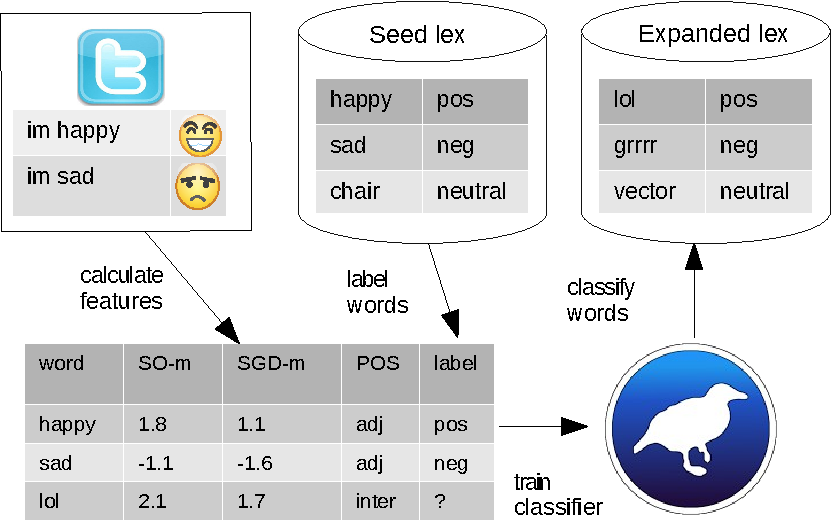
\includegraphics[scale=0.8]{diagram_crop.pdf}
	\label{fig:sosgd}
\end{figure}


\end{frame}





\begin{frame}{Obtaining Emoticon-annotated Tweets}
\begin{scriptsize}
\begin{itemize}
\item We \textbf{require} a collection of tweets with their corresponding \textbf{polarity labels}. 
\item Tweets can be collected from the Twitter API.
\item Tweets exhibiting \textbf{positive :)} and \textbf{negative :(} emoticons are labelled according to the emoticon's polarity.
\item We consider \textbf{two}  collections of tweets covering multiple topics: The \textbf{Edinburgh corpus} (ED), and the \textbf{Stanford Sentiment corpus} (STS).
\end{itemize}

\begin{table}[htbp]
\begin{center}
\begin{tabular}{l|c|c}
\hline
 & ED & STS \\ \hline
Positive & $1,813,705$ & $800,000$  \\ 
Negative & $324,917$ & $800,000$  \\ \hline
Total & $2,138,622$ & $1,600,000$ \\ 
\end{tabular}
\end{center}
\caption{Collection statistics}
\label{tab:colstats}
\end{table}
\end{scriptsize}

\end{frame}


\begin{frame}{Word-level Attributes}
\begin{scriptsize}
\begin{itemize}
\item We calculate three type of word-level features to train the word-level classifier.

\item \textbf{SGD}: Are calculated from the weights of a \textbf{linear support vector machine} trained using words as attributes and emoticons as labels.
\begin{equation}\label{eq:sgd}
\frac{\lambda}{2}||w||^2+\sum [1- y (\mathbf{xw} +b) ]_{+}.
\end{equation}

\item \textbf{SO}: Are calculated from the point-wise mutual information between the words and the sentiment labels.

\begin{equation}
 \operatorname{PMI}(w_{i}, y)= \log_{2} \left ( \frac{Pr(w_{i} \wedge y)}{Pr(w_{i})Pr(y)} \right )
\end{equation}

\item \textbf{POS}: We also include the POS-tag of the word as a nominal attribute.

\item To create training data for machine learning, all the words \textbf{matching} the seed lexicon are \textbf{labelled} according to the lexicon's polarities.
\end{itemize}
\end{scriptsize}
\end{frame}




\begin{frame}{Feature Visualisation}
\begin{scriptsize}
\begin{figure}[htb]
	\centering
	 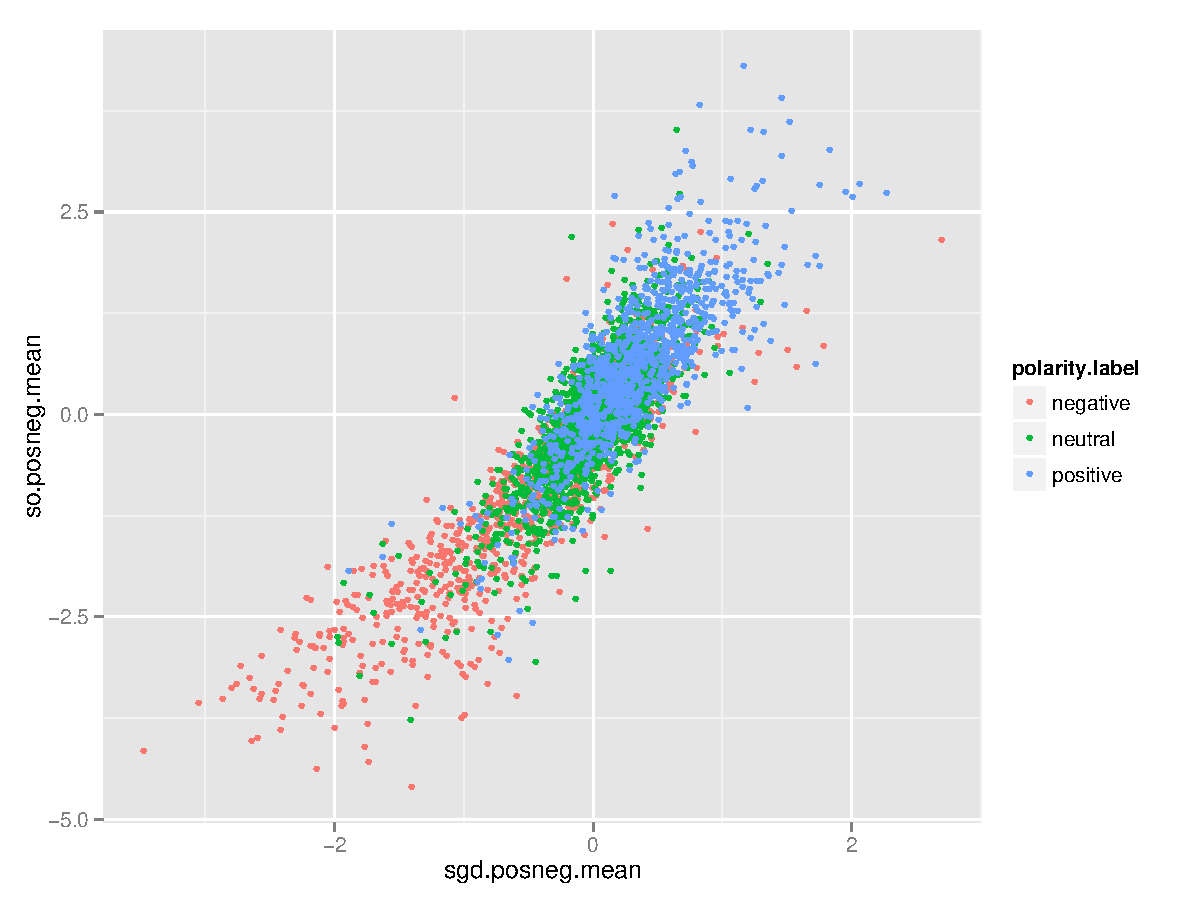
\includegraphics[width=7.5cm,height=6cm]{../SGDSO.pdf}
	\caption{SO vs SGD scatterplot.}
	\label{fig:sosgd}
\end{figure}
\end{scriptsize}

\end{frame}






\begin{frame}{Word-level Classification Results using RBF SVMs}
\footnotesize
\begin{table}[!htb]
\begin{center}
\begin{tabular}{l|l|l}
\hline \hline
\multicolumn{ 3}{c}{Weighted AUC } \\ \hline \hline
Dataset & SO & ALL \\ \hline
%ED-Neutrality & 0.62 $\pm$ 0.02 &  \textbf{0.65 $\pm$ 0.02} $\circ$ \\ 
%ED-PosNeg & 0.74 $\pm$ 0.03 & \textbf{0.75 $\pm$ 0.03} \\ 
ED-Polarity & 0.62 $\pm$ 0.02 &  \textbf{0.65 $\pm$0.02} $\circ$ \\ 
%STS-Neutrality & 0.63 $\pm$ 0.02 & \textbf{0.67 $\pm$ 0.02} $\circ$ \\ 
%STS-PosNeg & \textbf{0.77 $\pm$ 0.03} &  \textbf{0.77 $\pm$ 0.03} \\ 
STS-Polarity & 0.64 $\pm$ 0.02 & \textbf{0.66 $\pm$ 0.01} $\circ$   \\ \hline 
\hline \hline
\multicolumn{ 3}{c}{Kappa} \\ \hline \hline
Dataset & SO & ALL \\ \hline
%ED-Neutrality & 0.62 $\pm$ 0.02 &  \textbf{0.65 $\pm$ 0.02} $\circ$ \\ 
%ED-PosNeg & 0.74 $\pm$ 0.03 & \textbf{0.75 $\pm$ 0.03} \\ 
ED-Polarity & 0.28 $\pm$ 0.04 &  \textbf{0.33 $\pm$0.04} $\circ$ \\ 
%STS-Neutrality & 0.63 $\pm$ 0.02 & \textbf{0.67 $\pm$ 0.02} $\circ$ \\ 
%STS-PosNeg & \textbf{0.77 $\pm$ 0.03} &  \textbf{0.77 $\pm$ 0.03} \\ 
STS-Polarity & 0.31 $\pm$ 0.04 & \textbf{0.35 $\pm$ 0.03} $\circ$   \\ \hline 


\end{tabular}
\end{center}
\caption{World-level classification performance.} 
\label{tab:classres}
\end{table}


\end{frame}


\begin{frame}{Expanded Lexicon}
\begin{table}[htbp]
\scriptsize
\begin{tabular}{l|l|l|r|r|r}
\hline
word & POS & label & negative & neutral& positive \\ \hline
alrighty & interjection & positive & 0.021 & 0.087 & 0.892 \\ 
boooooo & interjection & negative & 0.984 & 0.013 & 0.003 \\ 
lmaoo & interjection & positive & 0.19 & 0.338 & 0.472 \\ 
french & adjective & neutral & 0.357 & 0.358 & 0.285 \\ 
handsome & adjective & positive & 0.007 & 0.026 & 0.968 \\ 
saddest & adjective & negative & 0.998 & 0.002 & 0 \\ 
same & adjective & negative & 0.604 & 0.195 & 0.201 \\ 
anniversary & common.noun & neutral & 0.074 & 0.586 & 0.339 \\ 
tear & common.noun & negative & 0.833 & 0.124 & 0.044 \\ 
relaxing & verb & positive & 0.064 & 0.244 & 0.692 \\ 
wikipedia & proper.noun & neutral & 0.102 & 0.644 & 0.254 \\ \hline
\end{tabular}
\caption{Expanded words example.}
\label{tab:expwords}
\end{table}
\end{frame}


\begin{frame}{Expanded Lexicon (2)}
\begin{figure}[ht]
\begin{center}
\begin{tabular}{cc}
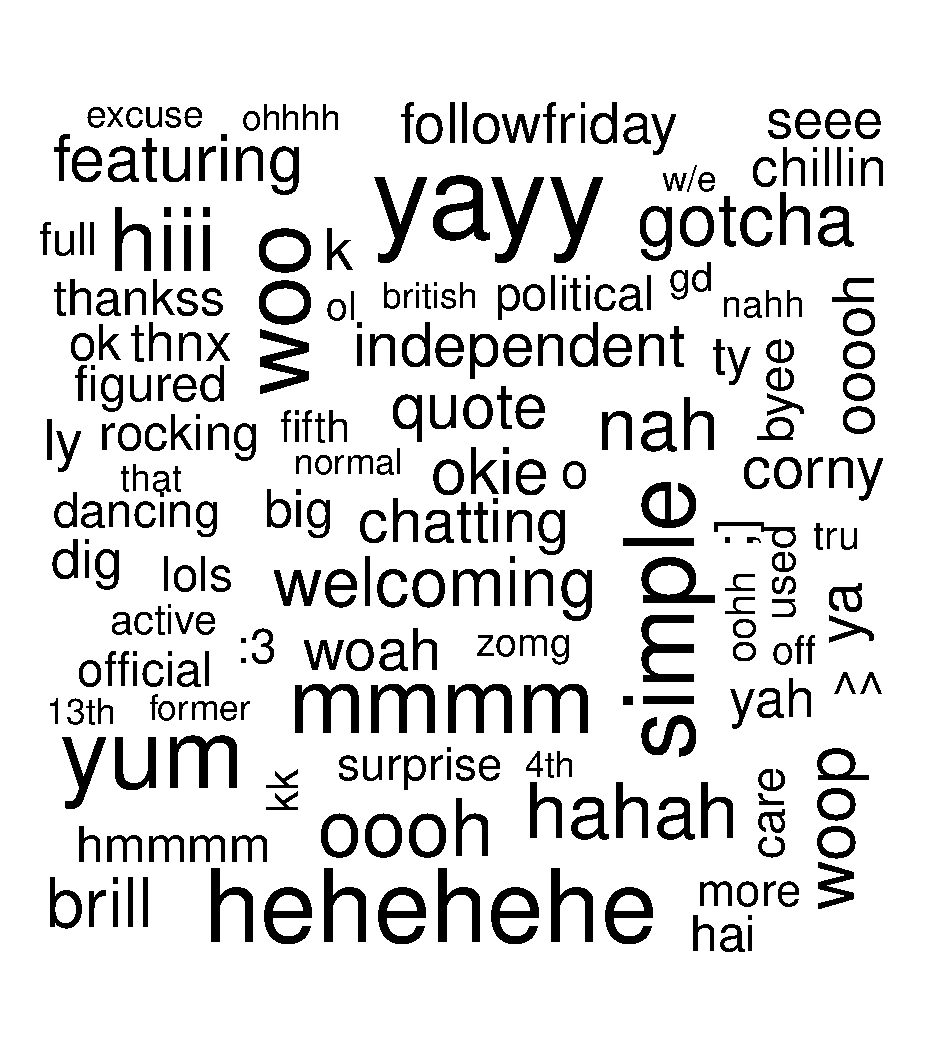
\includegraphics[scale=0.25]{../poswords.pdf}
&
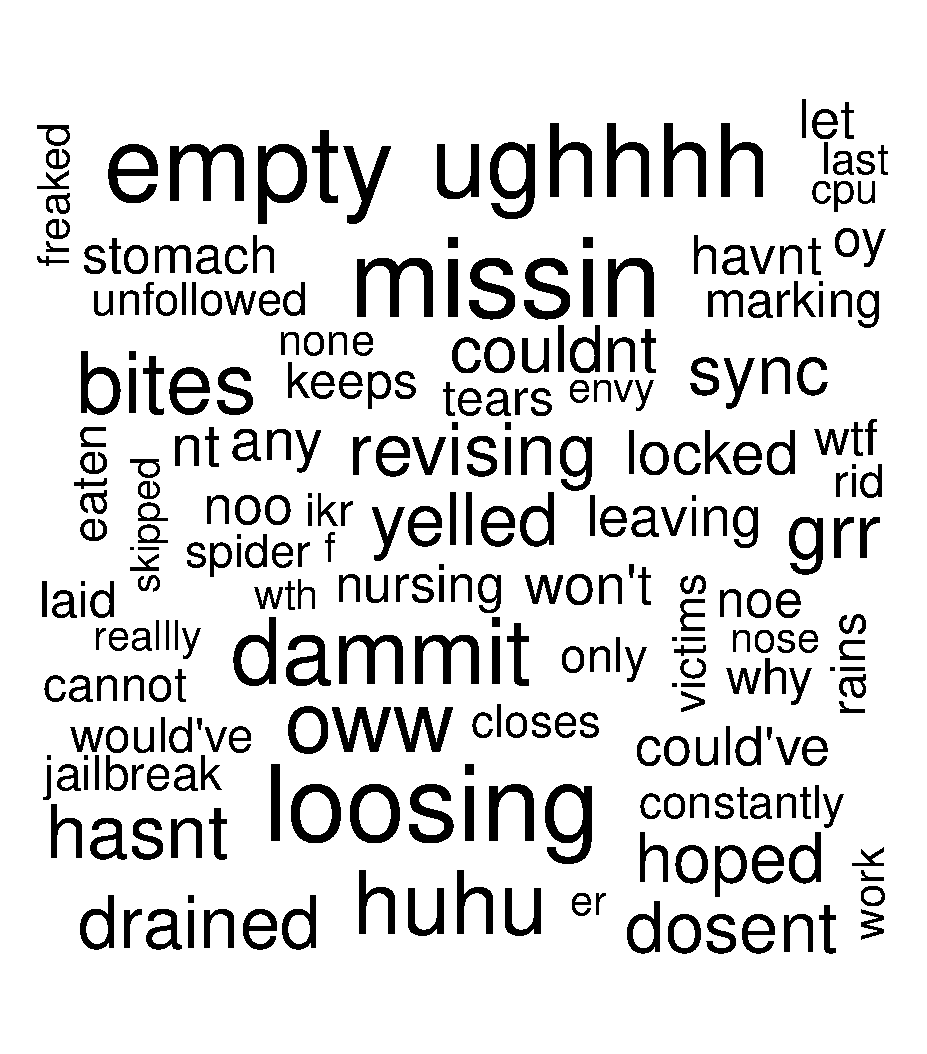
\includegraphics[scale=0.25]{../negwords.pdf}\\
(a) & (b)  
\end{tabular}
\caption{Word clouds of positive and negative words using log odds proportions.}
\label{fig:wordcloud}
\end{center}
\end{figure}
\end{frame}


\begin{frame}{Message-level Classification}
\footnotesize
\begin{table}[htbp]
\begin{center}
\begin{tabular}{l|l|l|l}
\hline \hline
\multicolumn{ 4}{c}{Weighted AUC } \\ \hline \hline
Dataset & Baseline & ED & STS  \\ \hline
6-coded & 0.77 $\pm$ 0.03 & 0.82 $\pm$ 0.03 $\circ$ & 0.82 $\pm$ 0.02 $\circ$  \\ 
Sanders & 0.77 $\pm$ 0.04 & 0.83 $\pm$ 0.04 $\circ$ & \textbf{0.84 $\pm$ 0.04} $\circ$  \\ 
SemEval & 0.77 $\pm$ 0.02 & 0.81 $\pm$ 0.02 $\circ$ & \textbf{0.83 $\pm$ 0.02} $\circ$ \\ \hline
\end{tabular}
\caption{Message-level polarity classification performance.}
\label{tab:messclass}
\end{center}
\end{table}
\end{frame}


\begin{frame}{Discussions}
\begin{scriptsize}
\begin{itemize}
\item This method could be used to create \textbf{domain-specific} lexicons.
\item It could also be used to study the \textbf{dynamics} of opinion-words.
\item This method depends on a collection of \textbf{emoticon-annotated tweets}.
\item It would be hard to apply to \textbf{domains} where emoticons are not \textbf{frequently used}.
\item Source code and lexicons available at \url{http://www.cs.waikato.ac.nz/ml/sa/lex.html}.
\item Feel free to visit me at poster \textbf{\#88}.

\end{itemize}
\end{scriptsize}

\end{frame}





\begin{frame}
\frametitle{Questions?}
%\vspace{1.5cm}
\begin{center}\LARGE Thanks for your Attention!\\ \end{center}

\begin{columns}
\begin{column}{0.55\textwidth}
\begin{block}{Acknowledgments}
\begin{itemize}\tiny
	\item University of Waikato Doctoral Scholarship
	\item Machine Learning Group at the University of Waikato
	
\end{itemize}
\end{block}
\end{column}
\begin{column}{0.45\textwidth}
\vspace{1.5cm}

\begin{figure}[h!]
	\centering
	\includegraphics[scale=0.3]{../../img/waikato.png}
\end{figure}
\end{column}
\end{columns}

\end{frame}




%%%%%%%%%%%%%%%%%%%%%%%%%%%

\end{document}
